\documentclass[14pt,compress,t,noamsthm,notheorem,table,handout,fontset=none]{ctexbeamer}

\setCJKmainfont[
  Path=/usr/local/texlive/2024/texmf-dist/fonts/opentype/public/fandol/,
  BoldFont=FandolSong-Bold.otf
]{FandolSong-Regular.otf}
\setCJKsansfont[
  Path=/usr/local/texlive/2024/texmf-dist/fonts/opentype/public/fandol/,
  BoldFont=FandolHei-Bold.otf
]{FandolHei-Regular.otf}
\setCJKmonofont[
  Path=/usr/local/texlive/2024/texmf-dist/fonts/opentype/public/fandol/
]{FandolFang-Regular.otf}

\setsansfont[
  Path=/usr/local/texlive/2024/texmf-dist/fonts/opentype/public/tex-gyre/,
  BoldFont=texgyreheros-bold.otf,
  ItalicFont=texgyreheros-italic.otf,
  BoldItalicFont=texgyreheros-bolditalic.otf
]{texgyreheros-regular.otf}
\setmonofont[
  Path=/usr/local/texlive/2024/texmf-dist/fonts/opentype/public/inconsolata/,
  BoldFont=Inconsolatazi4-Bold.otf,
  StylisticSet=3
]{Inconsolatazi4-Regular.otf}

\usetheme{default}
\usefonttheme[onlymath]{serif}
\setbeamertemplate{navigation symbols}{}

\usepackage{amsmath,amssymb}
\usepackage{booktabs}
\usepackage{graphicx}
\usepackage{hyperref}
\usepackage{listings}
\usepackage{xcolor}
\usepackage{etoolbox}

\graphicspath{{figs/}}
\definecolor{navy}{HTML}{193B5B}
\definecolor{bodytext}{HTML}{24313D}
\definecolor{muted}{HTML}{617080}
\definecolor{rulegray}{HTML}{CBD4DD}
\definecolor{codebg}{HTML}{F4F6F8}
\definecolor{codeframe}{HTML}{D5DDE5}
\definecolor{codecomment}{HTML}{4B705C}
\definecolor{codestring}{HTML}{92533C}
\definecolor{tablehead}{HTML}{EEF2F6}
\hypersetup{pdfborder=0 0 0,colorlinks=true,linkcolor=navy,urlcolor=navy}

\setbeamercolor{normal text}{fg=bodytext,bg=white}
\setbeamercolor{structure}{fg=navy}
\setbeamercolor{frametitle}{fg=navy,bg=white}
\setbeamercolor{myfootline}{bg=white,fg=muted}
\setbeamercolor{block title}{fg=navy,bg=white}
\setbeamercolor{block body}{fg=bodytext,bg=white}
\setbeamercolor{alerted text}{fg=codestring}
\setbeamerfont{frametitle}{size=\fontsize{18}{21},series=\bfseries}
\setbeamerfont{block title}{size=\normalsize,series=\bfseries}
\setbeamertemplate{blocks}[default]
\setbeamertemplate{itemize item}{\raisebox{0.15ex}{\scriptsize\textbullet}}
\setbeamertemplate{enumerate item}{\insertenumlabel.}
\AtBeginEnvironment{itemize}{\setlength{\itemsep}{0.24em}}
\AtBeginEnvironment{enumerate}{\setlength{\itemsep}{0.24em}}
\arrayrulecolor{rulegray}
\setlength{\heavyrulewidth}{0.6pt}
\setlength{\lightrulewidth}{0.35pt}

\setbeamertemplate{headline}{}
\setbeamertemplate{footline}{%
  \leavevmode\mbox{%
    \begin{beamercolorbox}[wd=.75\paperwidth,ht=3mm,dp=2mm,left]{myfootline}%
      \hspace*{0.8cm}{\fontsize{7.5}{9}\selectfont 统计学导论上机课}
    \end{beamercolorbox}%
    \begin{beamercolorbox}[wd=.25\paperwidth,ht=3mm,dp=2mm,right]{myfootline}%
      {\fontsize{7.5}{9}\selectfont\insertframenumber\,/\,\inserttotalframenumber\hspace*{0.8cm}}
    \end{beamercolorbox}}
  \vskip0pt}
\setbeamertemplate{frametitle}{%
  \vspace{0.28cm}%
  {\usebeamerfont{frametitle}\usebeamercolor[fg]{frametitle}\insertframetitle\par}%
  \vspace{0.12cm}%
  {\color{rulegray}\hrule height 0.45pt}%
  \vspace{-0.2cm}}
\setbeamersize{text margin left=0.8cm,text margin right=0.8cm}

\setbeamertemplate{title page}{%
  \vspace*{0.95cm}%
  {\fontsize{25}{31}\selectfont\bfseries\color{navy}\inserttitle\par}%
  \vspace{0.35cm}%
  {\fontsize{14}{19}\selectfont\color{bodytext}\insertsubtitle\par}%
  \vspace{0.65cm}%
  {\color{rulegray}\hrule height 0.45pt}%
  \vspace{0.6cm}%
  {\fontsize{13}{18}\selectfont\insertauthor\par}%
  \vspace{0.12cm}%
  {\fontsize{10}{15}\selectfont\color{muted}\insertinstitute\par}%
  \vfill
  {\fontsize{10}{14}\selectfont\color{muted}\insertdate\par}%
  \vspace*{0.6cm}}

\lstset{
  language=R,
  basicstyle=\ttfamily\fontsize{12.5}{14.5}\selectfont\color{bodytext},
  keywordstyle=\color{navy},
  commentstyle=\color{codecomment},
  stringstyle=\color{codestring},
  backgroundcolor=\color{codebg},
  frame=single,
  rulecolor=\color{codeframe},
  framerule=0.35pt,
  framesep=5pt,
  showstringspaces=false,
  keepspaces=true,
  breaklines=true,
  columns=fullflexible,
  xleftmargin=5pt,
  xrightmargin=5pt,
  aboveskip=0.35em,
  belowskip=0.35em
}

\lstdefinestyle{output}{
  language={},
  keywordstyle=\color{bodytext},
  commentstyle=\color{bodytext},
  stringstyle=\color{bodytext},
  backgroundcolor=\color{white},
  frame=none,
  aboveskip=0.12em,
  belowskip=0.25em
}

\newcommand{\code}[1]{\textcolor{navy}{\texttt{#1}}}
\newcommand{\inputlabel}{\par\smallskip{\fontsize{10.5}{13}\selectfont\bfseries\color{muted}输入代码\par}}
\newcommand{\outputlabel}{\par\smallskip{\fontsize{10.5}{13}\selectfont\bfseries\color{muted}Console 输出\par}}
\newcommand{\thead}[1]{\textcolor{navy}{\textbf{#1}}}

\title{R语言基础（三）}
\subtitle{基本运算、常用函数与逻辑运算}
\author{郑泽靖}
\institute{北京师范大学统计学院}
\date{2026年秋季学期}

\begin{document}

\begin{frame}[plain]
  \titlepage
  \note{教材第28--31、94--98页。本讲两节，每节45分钟。第一节讲运算与函数，第二节讲关系运算、逻辑运算与抽样。}
\end{frame}

\begin{frame}[fragile]{上讲回顾：数据结构与列表}
  \small
  \renewcommand{\arraystretch}{1.15}
  \begin{tabular*}{\linewidth}{@{\extracolsep{\fill}}ll@{}}
    \toprule
    \thead{数据结构} & \thead{基本用途} \\
    \midrule
    向量 & 保存一组同类型的值 \\
    矩阵 & 按行和列组织同类型的值 \\
    数据框 & 按列保存一张数据表 \\
    列表 & 组合不同的 R 对象 \\
    \bottomrule
  \end{tabular*}
  \inputlabel
\begin{lstlisting}
lst <- list(u = 2, v = "abcd")
lst[[1]]
names(lst) <- c("num", "string")
\end{lstlisting}
  \code{lst[[1]]} 得到 2；更名后用 \code{lst\$num} 提取该分量。
  \note{教材第19--27页。第一节第0--3分钟，复习3分钟。创建、提取和更名仅作回顾，不重新展开列表。}
\end{frame}

\begin{frame}[fragile]{矩阵运算：准备数据}
  后面几页使用同一组矩阵 \code{A} 和 \code{B}。
  \begin{columns}[T,onlytextwidth]
    \begin{column}{0.48\textwidth}
      \inputlabel
\begin{lstlisting}
A <- matrix(1:4, 2, 2,
  byrow = TRUE)
A
\end{lstlisting}
      \outputlabel
\begin{lstlisting}[style=output]
     [,1] [,2]
[1,]    1    2
[2,]    3    4
\end{lstlisting}
    \end{column}
    \begin{column}{0.48\textwidth}
      \inputlabel
\begin{lstlisting}
B <- matrix(
  c(2, 5, 3, 6), 2, 2)
B
\end{lstlisting}
      \outputlabel
\begin{lstlisting}[style=output]
     [,1] [,2]
[1,]    2    3
[2,]    5    6
\end{lstlisting}
    \end{column}
  \end{columns}
  \note{教材第28页。运算与求和共17分钟，第一节第3--20分钟。先检查矩阵A按行、B按列填入，后面沿用这两个对象。}
\end{frame}

\begin{frame}[fragile]{同型矩阵的加减}
  行数和列数相同的矩阵，按对应位置进行加减。
  \begin{columns}[T,onlytextwidth]
    \begin{column}{0.48\textwidth}
      \inputlabel
\begin{lstlisting}
A + B
\end{lstlisting}
      \outputlabel
\begin{lstlisting}[style=output]
     [,1] [,2]
[1,]    3    5
[2,]    8   10
\end{lstlisting}
    \end{column}
    \begin{column}{0.48\textwidth}
      \inputlabel
\begin{lstlisting}
A - B
\end{lstlisting}
      \outputlabel
\begin{lstlisting}[style=output]
     [,1] [,2]
[1,]   -1   -1
[2,]   -2   -2
\end{lstlisting}
    \end{column}
  \end{columns}
  \par\vspace{0.4em}
  例如，\code{A + B} 左上角的结果为 $1+2=3$。
  \note{教材第28--29页。对应表1-3的加减运算。只手算左上角，其他位置用相同规则核对。}
\end{frame}

\begin{frame}[fragile]{矩阵与一个数的加减}
  一个数与矩阵运算时，\par
  分别作用于矩阵中的每个元素。
  \begin{columns}[T,onlytextwidth]
    \begin{column}{0.48\textwidth}
      \inputlabel
\begin{lstlisting}
A + 2
\end{lstlisting}
      \outputlabel
\begin{lstlisting}[style=output]
     [,1] [,2]
[1,]    3    4
[2,]    5    6
\end{lstlisting}
    \end{column}
    \begin{column}{0.48\textwidth}
      \inputlabel
\begin{lstlisting}
2 - A
\end{lstlisting}
      \outputlabel
\begin{lstlisting}[style=output]
     [,1] [,2]
[1,]    1    0
[2,]   -1   -2
\end{lstlisting}
    \end{column}
  \end{columns}
  \par\vspace{0.4em}
  \code{2 - A} 在每个位置都用 2 减去原来的元素。
  \note{教材第28页表1-3、第29页A+2。2-A是表中数减矩阵规则的直接应用，提醒减法的先后顺序。}
\end{frame}

\begin{frame}[fragile]{按元素相乘与相除}
  \code{*} 和 \code{/} 对矩阵中相同位置的元素进行运算。
  \begin{columns}[T,onlytextwidth]
    \begin{column}{0.43\textwidth}
      \inputlabel
\begin{lstlisting}
A * B
\end{lstlisting}
      \outputlabel
\begin{lstlisting}[style=output]
     [,1] [,2]
[1,]    2    6
[2,]   15   24
\end{lstlisting}
    \end{column}
    \begin{column}{0.53\textwidth}
      \inputlabel
\begin{lstlisting}
A / B
\end{lstlisting}
      \outputlabel
\begin{lstlisting}[style=output]
     [,1]      [,2]
[1,]  0.5 0.6666667
[2,]  0.6 0.6666667
\end{lstlisting}
    \end{column}
  \end{columns}
  \par\vspace{0.4em}
  本例两矩阵的行数、列数分别相同。
  \note{教材第28--29页。A*B为对应位置相乘；A/B为对应位置相除。提前说明矩阵乘法使用后面的另一个符号。}
\end{frame}

\begin{frame}[fragile]{按元素进行幂运算}
  \code{A\textasciicircum 2} 计算每个元素的平方。\par
  \code{A\textasciicircum B} 用 \code{B} 中对应元素作为指数。
  \begin{columns}[T,onlytextwidth]
    \begin{column}{0.48\textwidth}
      \inputlabel
\begin{lstlisting}
A ^ 2
\end{lstlisting}
      \outputlabel
\begin{lstlisting}[style=output]
     [,1] [,2]
[1,]    1    4
[2,]    9   16
\end{lstlisting}
    \end{column}
    \begin{column}{0.48\textwidth}
      \inputlabel
\begin{lstlisting}
A ^ B
\end{lstlisting}
      \outputlabel
\begin{lstlisting}[style=output]
     [,1] [,2]
[1,]    1    8
[2,]  243 4096
\end{lstlisting}
    \end{column}
  \end{columns}
  \note{教材第28--29页。以右下角4的6次幂等于4096说明矩阵指数也是按元素计算。不引入矩阵幂的推导。}
\end{frame}

\begin{frame}[fragile]{矩阵与一个数的除法}
  \begin{columns}[T,onlytextwidth]
    \begin{column}{0.48\textwidth}
      \inputlabel
\begin{lstlisting}
C <- matrix(1:6, 2, 3,
  byrow = TRUE)
C
\end{lstlisting}
      \outputlabel
\begin{lstlisting}[style=output]
     [,1] [,2] [,3]
[1,]    1    2    3
[2,]    4    5    6
\end{lstlisting}
    \end{column}
    \begin{column}{0.48\textwidth}
      \inputlabel
\begin{lstlisting}
C / 2
\end{lstlisting}
      \outputlabel
\begin{lstlisting}[style=output]
     [,1] [,2] [,3]
[1,]  0.5  1.0  1.5
[2,]  2.0  2.5  3.0
\end{lstlisting}
    \end{column}
  \end{columns}
  \par\vspace{0.3em}
  \code{C / 2} 将每个元素除以 2。\par
  \code{A} 是 $2\times2$，\code{C} 是 $2\times3$，不能直接相加。
  \note{教材第29页。C为教材例子。A+C、A*C、C/A均因维数不相容而报错，作为口头检查，不要求学生专门输入错误代码。}
\end{frame}

\begin{frame}[fragile]{矩阵乘法}
  \code{\%*\%} 表示矩阵乘法。\par
  左边矩阵的列数须等于右边矩阵的行数。
  \inputlabel
\begin{lstlisting}
A %*% C
\end{lstlisting}
  \outputlabel
\begin{lstlisting}[style=output]
     [,1] [,2] [,3]
[1,]    9   12   15
[2,]   19   26   33
\end{lstlisting}
  本例：$2\times2$ 的矩阵乘 $2\times3$ 的矩阵，\par
  得到 $2\times3$ 的矩阵。矩阵与一个数相乘使用 \code{*}。
  \note{教材第28--29页。教师演示约2分钟，说明符号和维数即可，不展开线性代数推导。矩阵与单个数相乘用普通乘号。}
\end{frame}

\begin{frame}[fragile]{矩阵求逆}
  \code{solve(A)} 计算矩阵 \code{A} 的逆矩阵。
  \inputlabel
\begin{lstlisting}
solve(A)
\end{lstlisting}
  \outputlabel
\begin{lstlisting}[style=output]
     [,1] [,2]
[1,] -2.0  1.0
[2,]  1.5 -0.5
\end{lstlisting}
  \begin{itemize}
    \item 求逆的对象须为可逆的方阵。
    \item 本例 \code{A} 可以求逆。\code{C} 不是方阵，不能这样求逆。
  \end{itemize}
  \note{教材第28--29页。教师演示约1分钟，只介绍solve(A)的用途与本例结果，不推导逆矩阵，也不增加方程求解用法。}
\end{frame}

\begin{frame}[fragile]{求和函数}
  \code{sum()} 计算所有元素之和。
  \inputlabel
\begin{lstlisting}
sum(c(1, 2, 3))
\end{lstlisting}
  \outputlabel
\begin{lstlisting}[style=output]
[1] 6
\end{lstlisting}
  接下来使用矩阵 \code{a}：
  \inputlabel
\begin{lstlisting}
a <- matrix(1:6, 2, 3, byrow = TRUE)
\end{lstlisting}
  \[
    a=\begin{pmatrix}1&2&3\\4&5&6\end{pmatrix}.
  \]
  \note{教材第29--30页。sum为基础复习。a与前页C数值相同，改用教材求和段落中的名称。用小写a，提醒大小写有区别。}
\end{frame}

\begin{frame}[fragile]{按行与按列求和}
  \begin{columns}[T,onlytextwidth]
    \begin{column}{0.48\textwidth}
      \code{rowSums()}：各行之和。
      \inputlabel
\begin{lstlisting}
rowSums(a)
\end{lstlisting}
      \outputlabel
\begin{lstlisting}[style=output]
[1]  6 15
\end{lstlisting}
      第一行：$1+2+3=6$。\par
      第二行：$4+5+6=15$。
    \end{column}
    \begin{column}{0.48\textwidth}
      \code{colSums()}：各列之和。
      \inputlabel
\begin{lstlisting}
colSums(a)
\end{lstlisting}
      \outputlabel
\begin{lstlisting}[style=output]
[1] 5 7 9
\end{lstlisting}
      三列分别得到 5、7、9。
    \end{column}
  \end{columns}
  \par\vspace{0.4em}
  两个函数都返回向量。
  \note{教材第29--30页。至此完成第一节第3--20分钟的运算与求和17分钟。用输出元素个数检查行和与列和是否混淆。}
\end{frame}

\begin{frame}[fragile]{数学函数作用于向量}
  数学函数可以逐个计算向量中的元素。\par
  \code{sin()} 计算正弦值，输入角度以弧度为单位。
  \inputlabel
\begin{lstlisting}
x <- seq(1, 11, 2)
sin(x)
\end{lstlisting}
  \outputlabel
\begin{lstlisting}[style=output]
[1]  0.8414710  0.1411200 -0.9589243
[4]  0.6569866  0.4121185 -0.9999902
\end{lstlisting}
  结果与 \code{x} 一一对应，仍是一个向量。\par
  输出中的 \code{[4]} 表示该行从第 4 个元素开始。
  \note{教材第30页。数学函数与绘图共12分钟，第一节第20--32分钟。沿教材正弦例说明向量化计算，不另列函数清单。}
\end{frame}

\begin{frame}[fragile]{数学函数作用于矩阵}
  当输入为矩阵时，\code{sin()} 对各位置分别计算，\par
  并保留原来的行数和列数。
  \inputlabel
\begin{lstlisting}
x <- seq(1, 11, 2)
x <- matrix(x, 2, 3)
sin(x)
\end{lstlisting}
  \outputlabel
\begin{lstlisting}[style=output]
         [,1]       [,2]       [,3]
[1,] 0.841471 -0.9589243  0.4121185
[2,] 0.141120  0.6569866 -0.9999902
\end{lstlisting}
  \note{教材第30页。提醒matrix默认按列填入，因此矩阵输出顺序与前页向量显示顺序不同。没有引入新的数学函数。}
\end{frame}

\begin{frame}[fragile]{绘制函数曲线}
  在平面上绘图，先准备每个点的横坐标与纵坐标。
  \inputlabel
\begin{lstlisting}
x <- seq(0, 10, 0.1)
y <- sin(x)
plot(x, y, type = "l")
\end{lstlisting}
  \begin{itemize}
    \item \code{x}：从 0 到 10，步长为 0.1。
    \item \code{y}：各个横坐标对应的正弦值。
    \item \code{type = "l"}：用线连接这些点，字母为小写 L。
  \end{itemize}
  图形显示在 RStudio 的 Plots 窗格中。
  \note{教材第31页。只讲教材中的x、y、type三个参数。先逐行运行，再切到Plots观察。需要时用?plot查看帮助，不增加图形参数。}
\end{frame}

\begin{frame}{正弦曲线的运行结果}
  \centering
  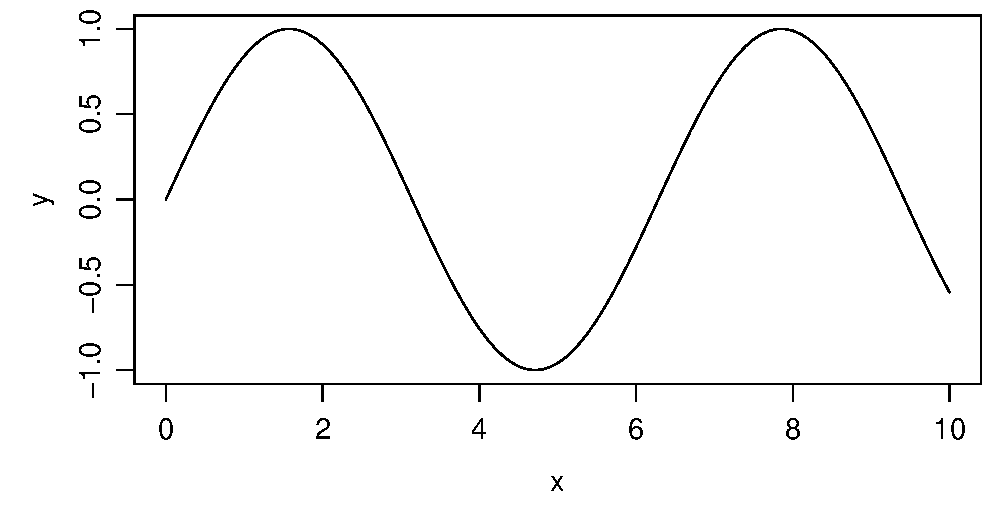
\includegraphics[width=0.94\linewidth,height=0.65\textheight,keepaspectratio]{sin-curve.pdf}
  \par\vspace{0.2em}
  \raggedright
  曲线对应上一页的 \code{plot(x, y, type = "l")}。\par
  Plots 窗格的 Export 可保存或复制图形。
  \note{教材第31页。图由上一页同一组x、y数据实际生成。至此完成第一节第20--32分钟的数学函数与绘图12分钟。Export沿教材说明，仅指认按钮，不扩展导出参数。}
\end{frame}

\begin{frame}{课堂练习一}
  练习时间：9 分钟。新建脚本 \code{R3-practice.R}。
  \begin{enumerate}
    \item 按行创建 $2\times3$ 矩阵 \code{M}，填入 1 到 6。\par
      计算 \mbox{\code{M + 2}}。
    \item 分别计算 \code{M} 的各行之和、各列之和。
    \item 创建从 0 到 10、步长为 0.1 的向量 \code{x}。\par
      计算 \mbox{\code{y = sin(x)}}，绘制折线图。
  \end{enumerate}
  \par\vspace{0.4em}
  在脚本中分段保存代码，运行后核对数值与图形。
  \note{教材第29--31页的课堂变式。第一节第32--41分钟，独立练习9分钟。仅使用已讲过的创建、加法、求和与绘图。无需提交。}
\end{frame}

\begin{frame}[fragile]{练习一参考：矩阵运算与求和}
  \inputlabel
\begin{lstlisting}
M <- matrix(1:6, 2, 3, byrow = TRUE)
M + 2
rowSums(M)
colSums(M)
\end{lstlisting}
  \small
  \renewcommand{\arraystretch}{1.2}
  \begin{tabular*}{\linewidth}{@{\extracolsep{\fill}}ll@{}}
    \toprule
    \thead{计算} & \thead{结果} \\
    \midrule
    \code{M + 2} & 两行分别为 3、4、5 和 6、7、8 \\
    \code{rowSums(M)} & 6、15 \\
    \code{colSums(M)} & 5、7、9 \\
    \bottomrule
  \end{tabular*}
  \note{教材第29--30页。与后两页合计第一节第41--45分钟讲评4分钟。主要检查byrow和两个求和函数，参考代码可独立运行。}
\end{frame}

\begin{frame}[fragile]{练习一参考：函数与绘图}
  \inputlabel
\begin{lstlisting}
x <- seq(0, 10, 0.1)
y <- sin(x)
plot(x, y, type = "l")
\end{lstlisting}
  \begin{itemize}
    \item 横坐标范围应为 0 到 10。
    \item 曲线应与前面的正弦曲线一致。
    \item \code{x} 与 \code{y} 的元素个数应相同。
  \end{itemize}
  \note{教材第30--31页。仍属第一节讲评4分钟，不再组织第二轮练习。检查type中的字母l和引号。}
\end{frame}

\begin{frame}{第一节操作核对}
  \small
  \renewcommand{\arraystretch}{1.25}
  \begin{tabular*}{\linewidth}{@{\extracolsep{\fill}}ll@{}}
    \toprule
    \thead{操作} & \thead{核对要点} \\
    \midrule
    \code{A * B} & 对应位置的元素相乘 \\
    \code{A \%*\% C} & 左边列数等于右边行数 \\
    \code{rowSums(a)} & 每行得到一个和 \\
    \code{colSums(a)} & 每列得到一个和 \\
    \code{sin(x)} & 对各个元素计算正弦值 \\
    \code{plot(x, y, type = "l")} & 在 Plots 窗格显示曲线 \\
    \bottomrule
  \end{tabular*}
  \par\vspace{0.5em}
  保存脚本 \code{R3-practice.R}。
  \note{教材第28--31页。第一节第45分钟结束。仅用表格核对典型错误，不逐页重讲。}
\end{frame}

\begin{frame}{关系运算符}
  关系运算判断两个值之间的关系，结果为\par
  \code{TRUE} 或 \code{FALSE}。
  \par\vspace{0.4em}
  \renewcommand{\arraystretch}{1.2}
  \begin{tabular*}{\linewidth}{@{\extracolsep{\fill}}ll@{}}
    \toprule
    \thead{运算符} & \thead{含义} \\
    \midrule
    \code{<} & 小于 \\
    \code{<=} & 小于或等于 \\
    \code{>} & 大于 \\
    \code{>=} & 大于或等于 \\
    \code{==} & 等于 \\
    \code{!=} & 不等于 \\
    \bottomrule
  \end{tabular*}
  \note{教材第94页表2-2。第二节第0--8分钟，关系运算8分钟，包含本页及后两页。提醒==用于比较，与<-赋值区分。}
\end{frame}

\begin{frame}[fragile]{向量的关系运算}
  向量与一个数比较时，对各个元素分别判断。
  \inputlabel
\begin{lstlisting}
X <- 1:5
X <= 4
\end{lstlisting}
  \outputlabel
\begin{lstlisting}[style=output]
[1]  TRUE  TRUE  TRUE  TRUE FALSE
\end{lstlisting}
  \par\vspace{0.3em}
  原向量 \code{X} 仍是 1、2、3、4、5。\par
  比较结果是与 \code{X} 等长的逻辑向量。
  \note{教材第94页。让学生把每一个TRUE/FALSE对应回原来的元素。关系运算也可用于矩阵，稍后逻辑矩阵中演示。}
\end{frame}

\begin{frame}[fragile]{字符的相等判断}
  \inputlabel
\begin{lstlisting}
b <- "abc"
other <- b
b == "abc"
b == "ab"
b == other
\end{lstlisting}
  \outputlabel
\begin{lstlisting}[style=output]
[1] TRUE
[1] FALSE
[1] TRUE
\end{lstlisting}
  字符值需要放在引号中。
  \note{教材第94页。other替代书中变量c，避免覆盖常用函数名。到此完成第二节第0--8分钟的关系运算。}
\end{frame}

\begin{frame}{逻辑运算符}
  \small
  \renewcommand{\arraystretch}{1.3}
  \begin{tabular*}{\linewidth}{@{\extracolsep{\fill}}lll@{}}
    \toprule
    \thead{运算符} & \thead{含义} & \thead{示例及结果} \\
    \midrule
    \code{!} & 非 & \code{!TRUE} 为 \code{FALSE} \\
             &    & \code{!FALSE} 为 \code{TRUE} \\
    \code{\&} & 与 & 两个条件都为真，结果才为真 \\
    \code{|} & 或 & 至少一个条件为真，结果为真 \\
    \bottomrule
  \end{tabular*}
  \par\vspace{0.6em}
  \begin{tabular*}{\linewidth}{@{\extracolsep{\fill}}llll@{}}
    \toprule
    & \code{TRUE, TRUE} & \code{TRUE, FALSE} & \code{FALSE, FALSE} \\
    \midrule
    \code{\&} & \code{TRUE} & \code{FALSE} & \code{FALSE} \\
    \code{|} & \code{TRUE} & \code{TRUE} & \code{FALSE} \\
    \bottomrule
  \end{tabular*}
  \note{教材第97--98页。第二节第8--16分钟，逻辑运算8分钟。矩阵例子由教师演示，各页沿用同一组x、a、b，不要求每页全班同步输入。}
\end{frame}

\begin{frame}[fragile]{关系运算生成逻辑矩阵}
  \begin{columns}[T,onlytextwidth]
    \begin{column}{0.48\textwidth}
      \inputlabel
\begin{lstlisting}
x <- matrix(1:6, 2, 3)
x
\end{lstlisting}
      \outputlabel
\begin{lstlisting}[style=output]
     [,1] [,2] [,3]
[1,]    1    3    5
[2,]    2    4    6
\end{lstlisting}
    \end{column}
    \begin{column}{0.48\textwidth}
      \inputlabel
\begin{lstlisting}
a <- x <= 3
a
\end{lstlisting}
      \outputlabel
\begin{lstlisting}[style=output]
      [,1]  [,2]  [,3]
[1,]  TRUE  TRUE FALSE
[2,]  TRUE FALSE FALSE
\end{lstlisting}
    \end{column}
  \end{columns}
  \par\vspace{0.4em}
  逻辑矩阵保留原矩阵的行数、列数\par
  和位置对应关系。
  \note{教材第98页。先创建x，再将每个位置是否不大于3的判断保存为逻辑矩阵a。}
\end{frame}

\begin{frame}[fragile]{逻辑矩阵：条件与取反}
  \begin{columns}[T,onlytextwidth]
    \begin{column}{0.48\textwidth}
      \inputlabel
\begin{lstlisting}
b <- x > 2
b
\end{lstlisting}
      \outputlabel
\begin{lstlisting}[style=output]
      [,1]  [,2] [,3]
[1,] FALSE  TRUE TRUE
[2,] FALSE  TRUE TRUE
\end{lstlisting}
    \end{column}
    \begin{column}{0.48\textwidth}
      \inputlabel
\begin{lstlisting}
!a
\end{lstlisting}
      \outputlabel
\begin{lstlisting}[style=output]
      [,1]  [,2] [,3]
[1,] FALSE FALSE TRUE
[2,] FALSE  TRUE TRUE
\end{lstlisting}
    \end{column}
  \end{columns}
  \par\vspace{0.4em}
  \code{!a} 将 \code{a} 中的真、假逐个取反。
  \note{教材第98页。b是x>2，与a是不同条件。右列只改变逻辑值，不修改a本身。}
\end{frame}

\begin{frame}[fragile]{逻辑矩阵：与、或}
  \code{a} 表示 \code{x <= 3}，\code{b} 表示 \code{x > 2}。
  \begin{columns}[T,onlytextwidth]
    \begin{column}{0.48\textwidth}
      \inputlabel
\begin{lstlisting}
a & b
\end{lstlisting}
      \outputlabel
\begin{lstlisting}[style=output]
      [,1]  [,2]  [,3]
[1,] FALSE  TRUE FALSE
[2,] FALSE FALSE FALSE
\end{lstlisting}
      只有数值 3 同时满足。
    \end{column}
    \begin{column}{0.48\textwidth}
      \inputlabel
\begin{lstlisting}
a | b
\end{lstlisting}
      \outputlabel
\begin{lstlisting}[style=output]
     [,1] [,2] [,3]
[1,] TRUE TRUE TRUE
[2,] TRUE TRUE TRUE
\end{lstlisting}
      所有位置至少满足一个。
    \end{column}
  \end{columns}
  \note{教材第98页。逐位置组合逻辑值。教材矩阵由1:6按列创建，两个条件同时为真只有第一行第二列，即数值3所在位置。}
\end{frame}

\begin{frame}[fragile]{矩阵与一个逻辑值}
  单个逻辑值也可以与逻辑矩阵中的各个元素运算。
  \begin{columns}[T,onlytextwidth]
    \begin{column}{0.48\textwidth}
      \inputlabel
\begin{lstlisting}
a & FALSE
\end{lstlisting}
      \outputlabel
\begin{lstlisting}[style=output]
      [,1]  [,2]  [,3]
[1,] FALSE FALSE FALSE
[2,] FALSE FALSE FALSE
\end{lstlisting}
    \end{column}
    \begin{column}{0.48\textwidth}
      \inputlabel
\begin{lstlisting}
a | FALSE
\end{lstlisting}
      \outputlabel
\begin{lstlisting}[style=output]
     [,1]  [,2]  [,3]
[1,] TRUE  TRUE FALSE
[2,] TRUE FALSE FALSE
\end{lstlisting}
    \end{column}
  \end{columns}
  \note{教材第98页a与F的运算。与FALSE运算全部为FALSE，或FALSE保留原逻辑值。教师快速展示，联系上一页真值表。}
\end{frame}

\begin{frame}[fragile]{单个条件的短路逻辑运算}
  \small
  \code{\&\&} 与 \code{||} 用于组合单个逻辑判断。
  \begin{columns}[T,onlytextwidth]
    \begin{column}{0.48\textwidth}
      \inputlabel
\begin{lstlisting}
n <- 2
(n <= 3) && (n > 2)
\end{lstlisting}
      \outputlabel
\begin{lstlisting}[style=output]
[1] FALSE
\end{lstlisting}
      \code{\&\&}：左侧为假时，\par
      不再计算右侧。
    \end{column}
    \begin{column}{0.48\textwidth}
      \inputlabel
\begin{lstlisting}
(n <= 3) || (n > 2)
\end{lstlisting}
      \outputlabel
\begin{lstlisting}[style=output]
[1] TRUE
\end{lstlisting}
      \code{||}：左侧为真时，\par
      不再计算右侧。
    \end{column}
  \end{columns}
  \par\vspace{0.3em}
  前面的逻辑向量、逻辑矩阵逐元素运算使用 \code{\&}、\code{|}。
  \note{教材第98页。短路逻辑运算两侧各为单个逻辑值。用n=2演示两个条件的与、或结果，不使用矩阵作为条件。到此第二节第16分钟。}
\end{frame}

\begin{frame}[fragile]{按条件提取向量元素}
  \code{X < 3} 先得到逻辑向量。\par
  将它放入方括号，提取对应 \code{TRUE} 的位置。
  \inputlabel
\begin{lstlisting}
X <- 1:5
X[X < 3]
\end{lstlisting}
  \outputlabel
\begin{lstlisting}[style=output]
[1] 1 2
\end{lstlisting}
  \par\vspace{0.3em}
  \code{X} 中小于 3 的元素为 1 和 2。
  \note{教材第94页。第二节第16--23分钟，条件提取与修改7分钟。前面已解释关系与逻辑运算，此处明确先判断、再提取的顺序。}
\end{frame}

\begin{frame}[fragile]{按条件修改向量元素}
  将 \code{X} 中小于 3 的元素统一改为 8。
  \inputlabel
\begin{lstlisting}
X <- 1:5
X[X < 3] <- 8
X
\end{lstlisting}
  \outputlabel
\begin{lstlisting}[style=output]
[1] 8 8 3 4 5
\end{lstlisting}
  \inputlabel
\begin{lstlisting}
X == 1:5
\end{lstlisting}
  \outputlabel
\begin{lstlisting}[style=output]
[1] FALSE FALSE  TRUE  TRUE  TRUE
\end{lstlisting}
  \note{教材第94页。教材X==1:5的逐位置比较用于核对修改后哪些位置仍与原值相同。赋值实际修改X，提醒后续例子按页重新创建X。}
\end{frame}

\begin{frame}[fragile]{组合两个筛选条件}
  提取大于或等于 2，并且小于或等于 4 的元素。
  \inputlabel
\begin{lstlisting}
X <- 1:5
X[(X >= 2) & (X <= 4)]
\end{lstlisting}
  \outputlabel
\begin{lstlisting}[style=output]
[1] 2 3 4
\end{lstlisting}
  \begin{itemize}
    \item 每个括号内先得到一个逻辑向量。
    \item \code{\&} 逐位置合并两个条件。
  \end{itemize}
  \note{教材第94、98页已有关系与逻辑运算的简单组合，不引入数据框筛选等新操作。到此完成第二节第16--23分钟的7分钟。}
\end{frame}

\begin{frame}[fragile]{随机抽样与 sample()}
  \small
  从 $1,\ldots,n$ 中等可能地取一个值，对应\par
  离散均匀分布：
  \[
    \mathrm{P}(X=k)=\frac{1}{n},\qquad k=1,\ldots,n.
  \]
  \code{sample()} 从给定向量中随机抽取元素。
  \inputlabel
% QA-TEMPLATE
\begin{lstlisting}
sample(x, size, replace = FALSE)
\end{lstlisting}
  \begin{itemize}
    \item \code{x}：供抽取的向量。
    \item \code{size}：抽取的个数。
    \item \code{replace}：是否有放回，默认 \code{FALSE}。
  \end{itemize}
  \note{教材第95页。第二节第23--32分钟，抽样与频率仍共9分钟。本页第23--25分钟，共2分钟。保留旧课件离散均匀分布定义，结合sample说明，不扩展其他概率分布。代码是调用格式，实际例子在下一页。}
\end{frame}

\begin{frame}[fragile]{有放回与不放回抽样}
  \inputlabel
\begin{lstlisting}
sample(1:10, 20, replace = TRUE)
sample(1:10, 5, replace = FALSE)
\end{lstlisting}
  \small
  \renewcommand{\arraystretch}{1.2}
  \begin{tabular*}{\linewidth}{@{\extracolsep{\fill}}lll@{}}
    \toprule
    \thead{抽样方式} & \thead{抽取个数} & \thead{本例结果的特点} \\
    \midrule
    有放回 & 20 & 来自 1 到 10，可重复 \\
    不放回 & 5 & 来自 1 到 10，互不重复 \\
    \bottomrule
  \end{tabular*}
  \par\vspace{0.5em}
  每次运行得到的具体数值和顺序可能不同。\par
  本例不放回时，最多只能抽取 10 个数。
  \note{教材第95页。第二节第25--27分钟，共2分钟。明确有放回允许重复，不能说一定重复每一个候选值。不放回的默认值为FALSE，sample(1:10,20)会报错。随机输出不与固定答案逐项比对。}
\end{frame}

\begin{frame}[fragile]{模拟掷骰子}
  每次掷一颗均匀骰子，对应从 1 到 6 中\par
  有放回地抽取一个数。
  \inputlabel
\begin{lstlisting}
dice <- sample(1:6, 100, replace = TRUE)
dice
\end{lstlisting}
  \begin{itemize}
    \item \code{dice} 保存 100 次模拟结果。
    \item 每个元素为 1、2、3、4、5、6 中的一个。
    \item 前面的结果不会使后面少一个可选点数。
  \end{itemize}
  运行后查看自己的结果，\par
  无需与教材数列逐项一致。
  \note{教材第95--96页。第二节第27--29分钟，共2分钟。与sample(1:6,100,T)含义相同，统一使用TRUE。dice替代全篇反复使用的x，便于与逻辑矩阵区分。为R-4掷骰重复实验做准备。}
\end{frame}

\begin{frame}[fragile]{出现次数与频率}
  \code{dice == 6} 判断每次是否出现 6。\par
  求和时，\code{TRUE} 按 1、\code{FALSE} 按 0 计算。
  \inputlabel
\begin{lstlisting}
sum(dice == 6)
sum(dice == 6) / 100
\end{lstlisting}
  \begin{itemize}
    \item 第一行：100 次中出现 6 的次数。
    \item 第二行：出现 6 的次数除以总次数，即频率。
  \end{itemize}
  频率随模拟结果变化，不要求恰好等于 $1/6$。
  \note{教材第97页。第二节第29--31分钟，共2分钟。仅用教材sum(逻辑条件)/实验次数计算某一面频率，不展开六面频率循环。TRUE/FALSE数值含义第一讲已学。下一页用1分钟演示教材硬币例，抽样与频率仍在第32分钟结束。}
\end{frame}

\begin{frame}[fragile]{硬币模拟：用 \texttt{mean()} 计算频率}
  用 1 表示正面、0 表示反面，模拟投掷一枚\par
  质地均匀的硬币 10000 次。
  \inputlabel
\begin{lstlisting}
x <- sample(c(0, 1), 10000, replace = TRUE)
mean(x)
\end{lstlisting}
  \code{mean(x)} 计算 \code{x} 中数值的平均数。
  \begin{itemize}
    \item 对于 0、1 数据，平均数等于 1 出现的频率。
    \item 本例结果是正面出现的频率，\par
      每次可能不同，不要求恰好等于 0.5。
  \end{itemize}
  \note{教材第95页硬币模拟原例。第二节第31--32分钟，共1分钟，仅教师演示。运行这两行代码，不显示10000个模拟值；只说明mean求平均数、0/1平均数即1的频率，不扩展均值理论、参数或练习。前四页各2分钟，本页1分钟，抽样与频率合计仍为9分钟。后续练习第32--41分钟、讲评第41--45分钟均不变。}
\end{frame}

\begin{frame}{课堂练习二}
  练习时间：9 分钟。在 \code{R3-practice.R} 中继续。
  \begin{enumerate}
    \item 创建 \code{X <- 1:10}，提取大于或等于 3、\par
      且小于或等于 7 的元素。
    \item 将 \code{X} 中小于 3 的元素改为 0，再显示 \code{X}。
    \item 模拟掷骰子 100 次，保存为 \code{dice}。计算出现 6 的次数和频率。
  \end{enumerate}
  \par\vspace{0.4em}
  前两题核对确定结果；\par
  第三题核对计算方法与结果范围。
  \note{教材第94--98页的课堂变式。第二节第32--41分钟，独立练习9分钟。均为已经讲过的向量操作，无数据框行筛选、循环或字符串生成。无需提交。}
\end{frame}

\begin{frame}[fragile]{练习二参考：条件提取与修改}
  \inputlabel
\begin{lstlisting}
X <- 1:10
X[(X >= 3) & (X <= 7)]
\end{lstlisting}
  \outputlabel
\begin{lstlisting}[style=output]
[1] 3 4 5 6 7
\end{lstlisting}
  \inputlabel
\begin{lstlisting}
X[X < 3] <- 0
X
\end{lstlisting}
  \outputlabel
\begin{lstlisting}[style=output]
[1]  0  0  3  4  5  6  7  8  9 10
\end{lstlisting}
  \note{教材第94、98页。第二节第41--45分钟，后三页讲评共4分钟。检查逐元素与单值逻辑运算是否混淆，比较用两个等号、赋值用左箭头。}
\end{frame}

\begin{frame}[fragile]{练习二参考：抽样与频率}
  \inputlabel
\begin{lstlisting}
dice <- sample(1:6, 100, replace = TRUE)
sum(dice == 6)
sum(dice == 6) / 100
\end{lstlisting}
  \begin{itemize}
    \item 出现次数应为 0 到 100 之间的整数。
    \item 频率为出现次数除以 100，介于 0 与 1 之间。
    \item 同学之间的结果可能不同，计算方法应一致。
  \end{itemize}
  \note{教材第95--97页。参考代码可独立运行。没有固定随机输出，重点核对replace=TRUE、==与总次数100。仍属于第二节讲评4分钟。}
\end{frame}

\begin{frame}{本讲操作核对}
  \small
  \renewcommand{\arraystretch}{1.3}
  \begin{tabular*}{\linewidth}{@{\extracolsep{\fill}}ll@{}}
    \toprule
    \thead{任务} & \thead{主要写法} \\
    \midrule
    比较值是否满足条件 & \code{<}、\code{<=}、\code{>}、\code{>=}、\code{==}、\code{!=} \\
    逐元素组合条件 & \code{!}、\code{\&}、\code{|} \\
    按条件提取、修改 & \code{X[\textsf{条件}]}、\code{X[\textsf{条件}] <- \textsf{新值}} \\
    随机抽样 & \code{sample(x, size, replace)} \\
    计算出现频率 & \code{sum(\textsf{条件}) / \textsf{总次数}} \\
    \bottomrule
  \end{tabular*}
  \par\vspace{0.5em}
  保存本讲脚本，下讲继续使用抽样与逻辑判断。
  \note{教材第94--98页。第二节第45分钟结束。保留课堂脚本，无提交作业要求。}
\end{frame}

\end{document}
